\documentclass{article}
\usepackage[utf8]{inputenc}
\usepackage[T1]{fontenc}
\usepackage[export]{adjustbox}
\usepackage{mathtools,amsthm,amssymb,icomma,upgreek,xfrac,enumerate, bbm,titlesec,lmodern,polski,derivative,geometry,multicol,titling,graphicx,url,amsmath,caption,lipsum,float,longtable,booktabs}
\usepackage[table,xcdraw]{xcolor}
\usepackage[hidelinks,breaklinks,pdfusetitle,pdfdisplaydoctitle]{hyperref}
\usepackage{listings}
\definecolor{codegreen}{rgb}{0,0.6,0}
\definecolor{codegray}{rgb}{0.5,0.5,0.5}
\definecolor{codepurple}{rgb}{0.58,0,0.82}
\definecolor{backcolour}{rgb}{0.95,0.95,0.92}
\definecolor{light-gray}{gray}{0.95}
\setlength{\droptitle}{-1cm}
\mathtoolsset{showonlyrefs,mathic}
\title{Analiza danych rzeczywistych przy pomocy modelu ARMA}
\author{Natalia Klepacka, Joanna Kołaczek}
\date{\today}
\newtheoremstyle{break}
{\topsep}{\topsep}%
{\normalfont}{}%
{\bfseries}{}%
{\newline}{}%
\theoremstyle{break}

\titleformat*{\section}{\LARGE\bfseries}
\titleformat*{\subsection}{\Large\bfseries}
\titleformat*{\subsubsection}{\large\bfseries}
\titleformat*{\paragraph}{\large\bfseries}
\titleformat*{\subparagraph}{\large\bfseries}

\lstdefinestyle{mystyle}{
	backgroundcolor=\color{backcolour},   
	commentstyle=\color{codegreen},
	keywordstyle=\color{magenta},
	numberstyle=\tiny\color{codegray},
	stringstyle=\color{codepurple},
	basicstyle=\ttfamily\footnotesize,
	breakatwhitespace=false,         
	breaklines=true,                 
	captionpos=b,                    
	keepspaces=true,                 
	numbers=left,                    
	numbersep=5pt,                  
	showspaces=false,                
	showstringspaces=false,
	showtabs=false,                  
	tabsize=2
}

\lstset{style=mystyle}
\renewcommand{\lstlistingname}{Kod}% Listing -> Kod
\renewcommand{\lstlistlistingname}{Lista Kodów}% List of Listings -> Lista kodów
\newcommand{\code}[1]{\colorbox{light-gray}{\texttt{#1}}}

\graphicspath{{obrazki/}}


\begin{document}
	\maketitle
	\tableofcontents
	\clearpage
	\section{Wstęp}
	Niniejszy raport powstał na potrzeby realizacji laboratorium z Komputerowej Analizy Szeregów Czasowych, prowadzonych przez mgr Justynę Witulską, do wykładu prof. Agnieszki Wyłomańskiej.
	Będziemy analizować dane dotyczące średniej dziennej temperatury w Londynnie, na przestrzeni lat 1979-2021. Dysponujemy 15304 obeserwacjami, jednak chcąc aby analiza była bardziej precyzyjna, będziemy rozważać tylko pierwszych 3040. Dane pochodzą \href{https://www.kaggle.com/datasets/emmanuelfwerr/london-weather-data }{\textit{z tej strony}}. Są to informacje kolekcjonowane przez European Climate Assessment and Dataset - projekt zbierający dane o pogodzie w Europie.
	W raporcie przyjrzymy się przebiegowi dekompozycji Walda, oraz przy pomocy kryteriów informacyjnych dobierzemy rzędy modelu ARMA aby następnie wyestymować wartości parametrów tegoż modelu. Zweryfikujemy również, czy założenia dotyczące szumu się zgadzają.

Życzymy Czytelnikowi miłej lektury.

\section{Przygotowanie danych do analizy}

Na wykresie [\ref{fig:p1}] przedstawiona jest zależność średniej dziennej temperatury w Londynie, w zależności od czasu. Wyraźnie widoczna jest sezonowość, natomiast nie możemy być pewni co do obecności trendu. Wykresy autokorelacji [\ref{fig:acf1}] oraz częściowej autokorelacji [\ref{fig:pacf1}] potwierdzają, że nie możemy mówić tu o szeregu stacjonarnym.

\begin{figure}[H]
	\begin{center}
		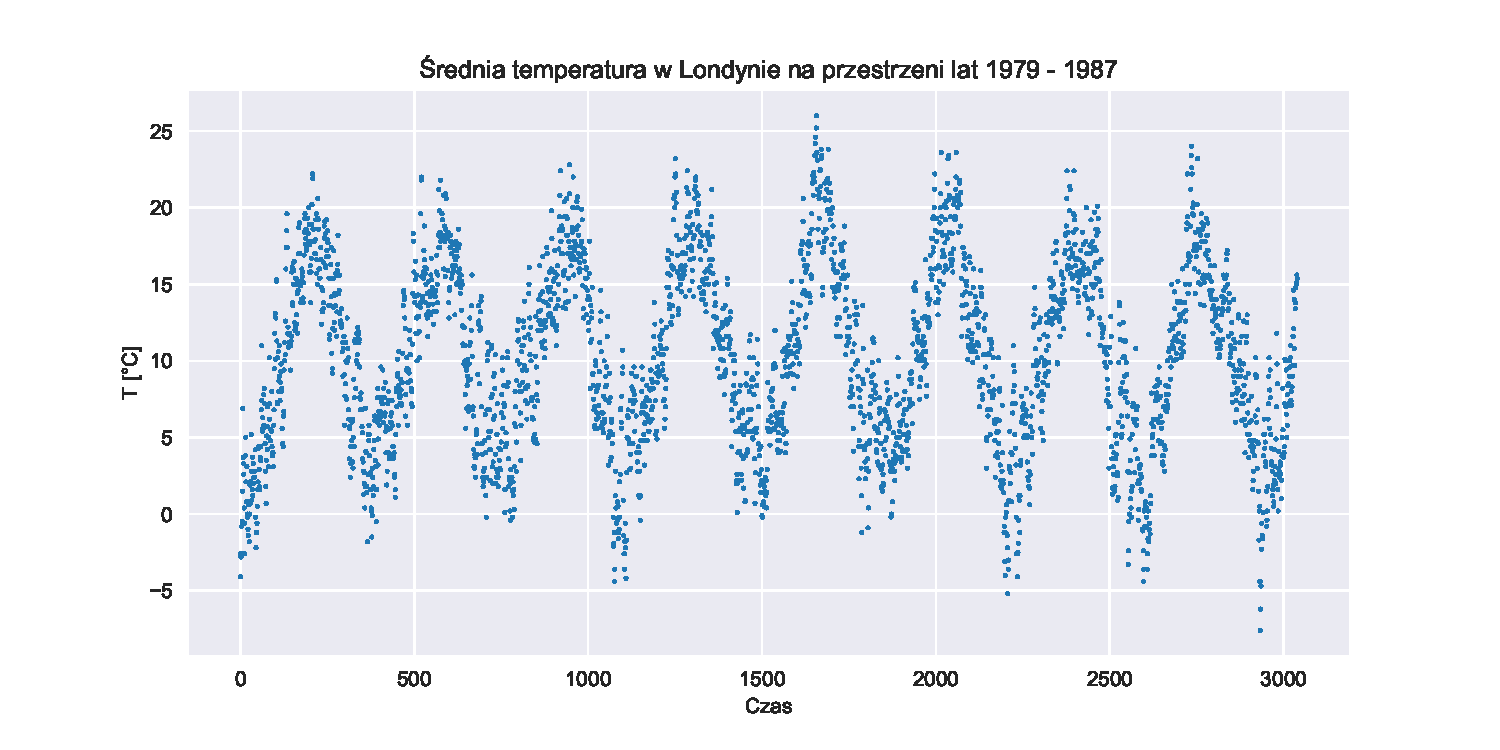
\includegraphics[scale=0.63]{plot1.pdf}
		\caption{Wykres temperatury w Londynie}
		\label{fig:p1}
	\end{center}
\end{figure}

	\begin{figure}[H]
	\begin{center}
		\begin{minipage}{0.49\linewidth}
			\centering
			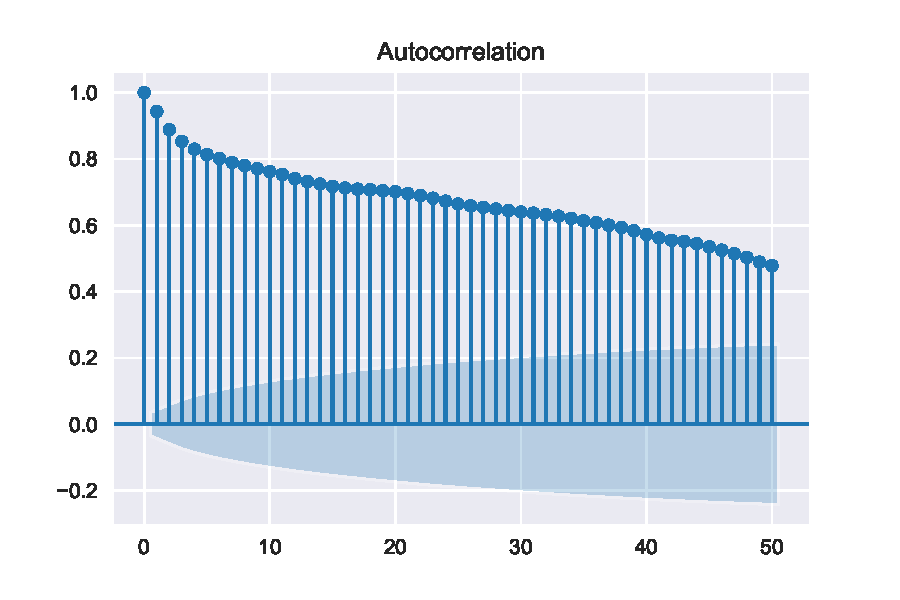
\includegraphics[scale=0.49]{acf1.pdf}
			\caption{Autokorelacja}
			\label{fig:acf1}
		\end{minipage}
		\begin{minipage}{0.49\linewidth}
			\centering
			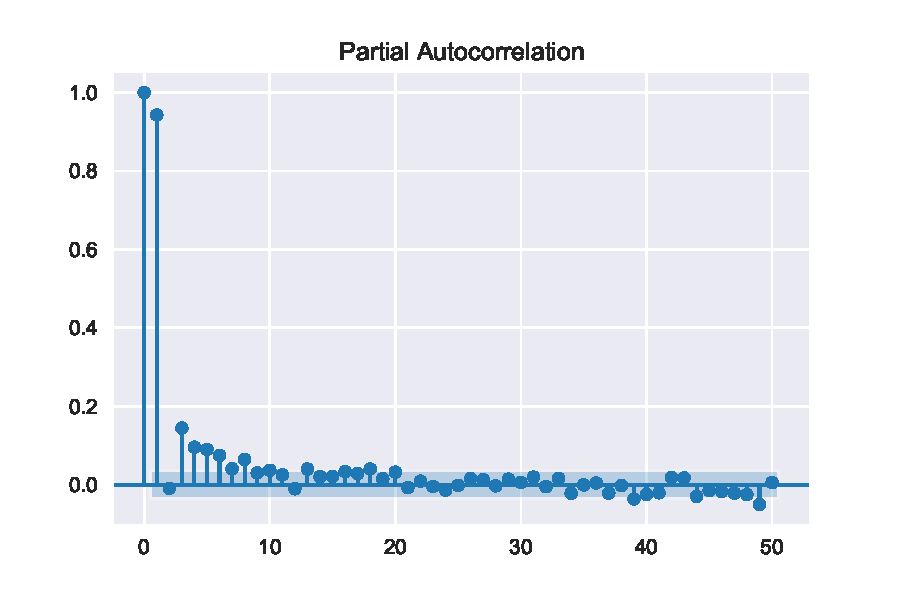
\includegraphics[scale=0.49]{pacf1.pdf}
			\caption{Częściowa autokorelacja}
			\label{fig:pacf1}
		\end{minipage}
	\end{center}
\end{figure}

Aby usunąć możliwy trend, stosujemy dla naszych danych regresję liniową. Efekt widzimy na wykresie [\ref*{fig:p2}]. Obliczony współczynnik kierunkowy był bardzo bliski zeru co oznacza, że w danych nie występuje trend liniowy, natomiast wyraz wolny wyniósł około 10, odejmujemy tą wartość od wartości oryginalnych aby je ustandaryzować. (?????????/)

\begin{figure}[H]
	\begin{center}
		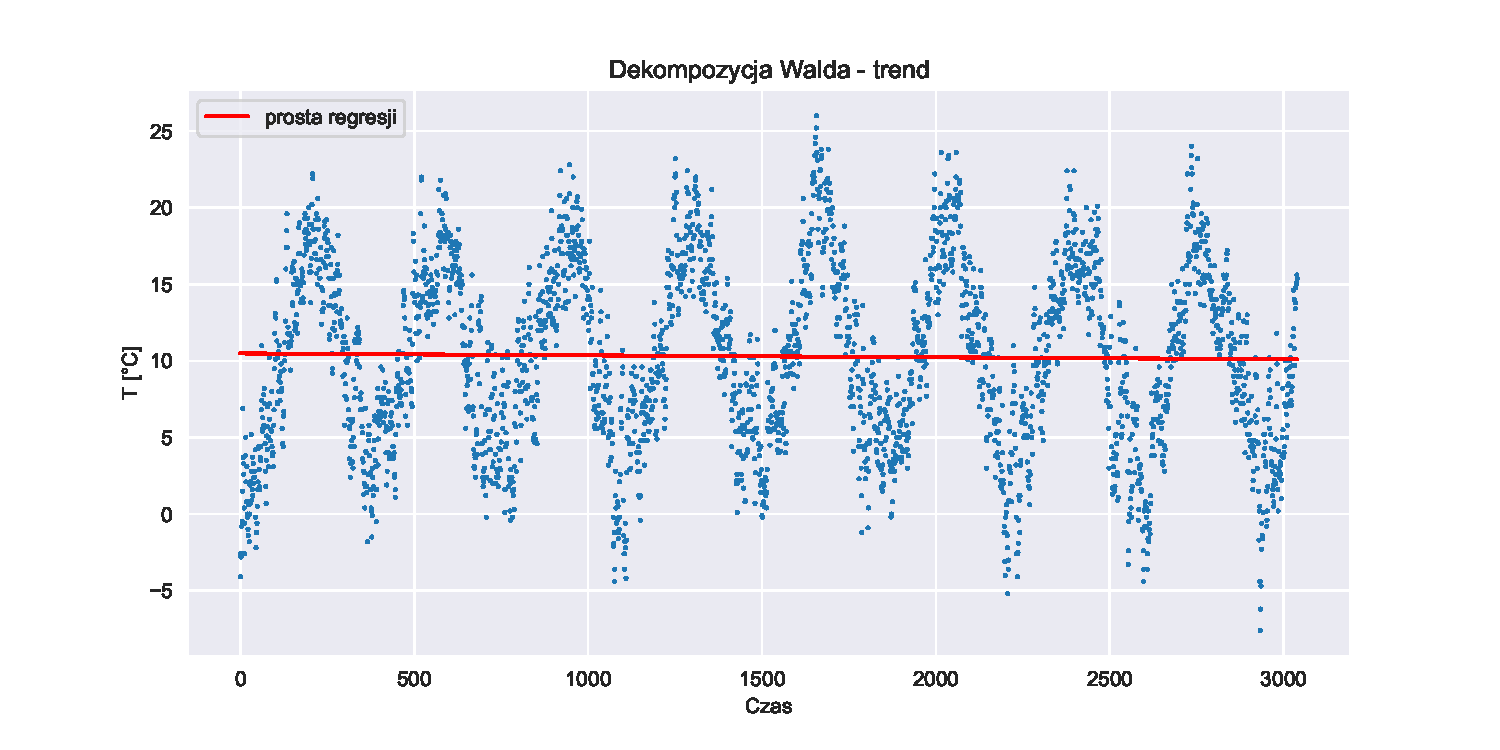
\includegraphics[scale=0.63]{plot2.pdf}
		\caption{Regresja liniowa}
		\label{fig:p2}
	\end{center}
\end{figure}

Kolejnym krokiem będzie próba usunięcia sezonowości. Na poprzednich wykresach mogliśmy zauważyć, że dane układają się w kształt funkcji sinusoidalnej. Załóżmy, że da się je opisać przy pomocy funkcji $f(x) = c\cdot\sin(d\cdot x+e)$. Używamy pakietu \code{scipy}, a konkretnie funkcji \code{optimize.curve\_fit}, aby dopasować odpowiednie współczynniki $c$, $d$, $e$. Efekt widzimy na wykresie \ref{fig:p3}.

\begin{figure}[H]
	\begin{center}
		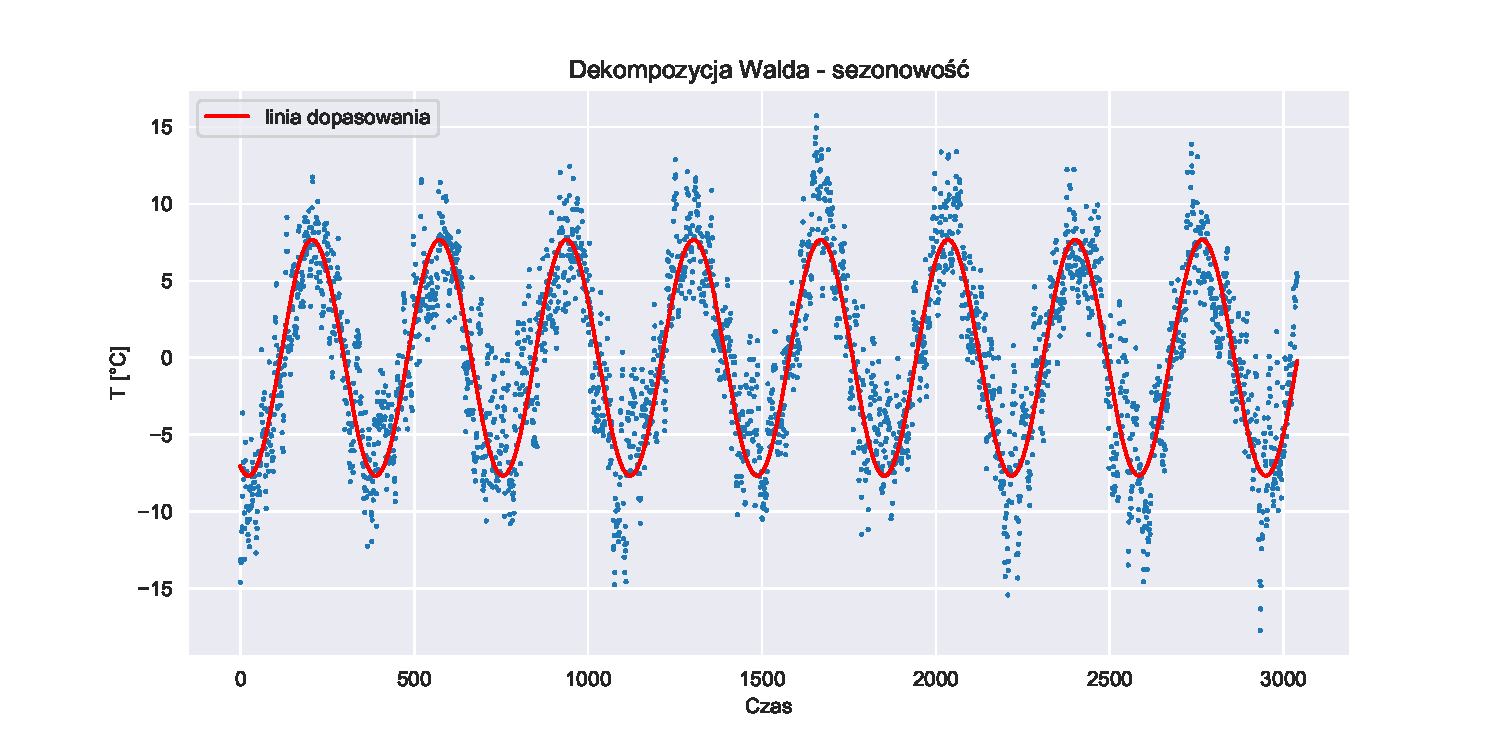
\includegraphics[scale=0.63]{plot3.pdf}
		\caption{Krzywa sinusoidalna}
		\label{fig:p3}
	\end{center}
\end{figure}

Aby dokończyć proces dekompozycji, wystarczy od naszych danych odjąć wartości otrzymanej funkcji w danym czasie [\ref{fig:p4}]. Możemy teraz ponownie sprawdzić jak prezentują się wykresy autokorelacji i częściowej autokorelacji. ...............

\begin{figure}[H]
	\begin{center}
		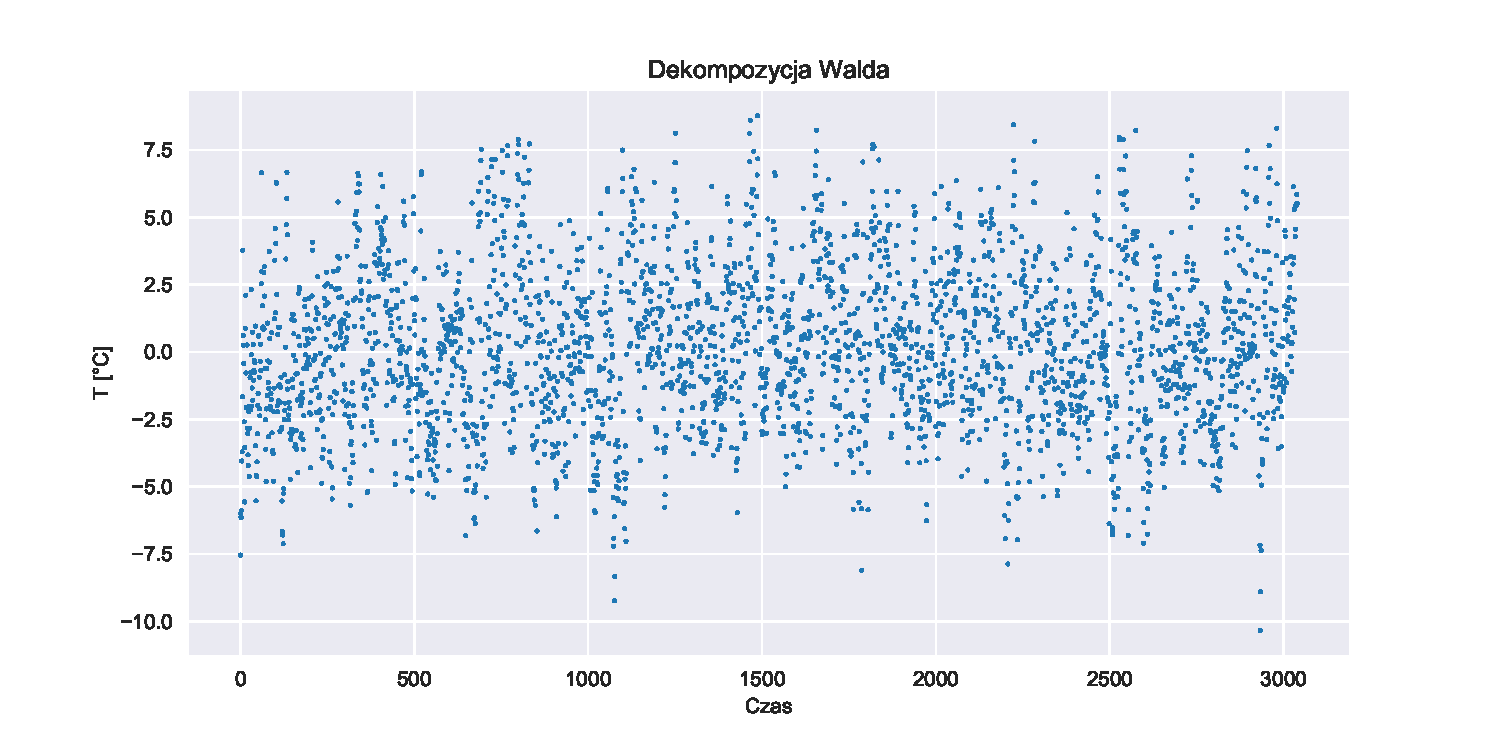
\includegraphics[scale=0.63]{plot4.pdf}
		\caption{Dane po dekompozycji}
		\label{fig:p4}
	\end{center}
\end{figure}

\begin{figure}[H]
	\begin{center}
		\begin{minipage}{0.49\linewidth}
			\centering
			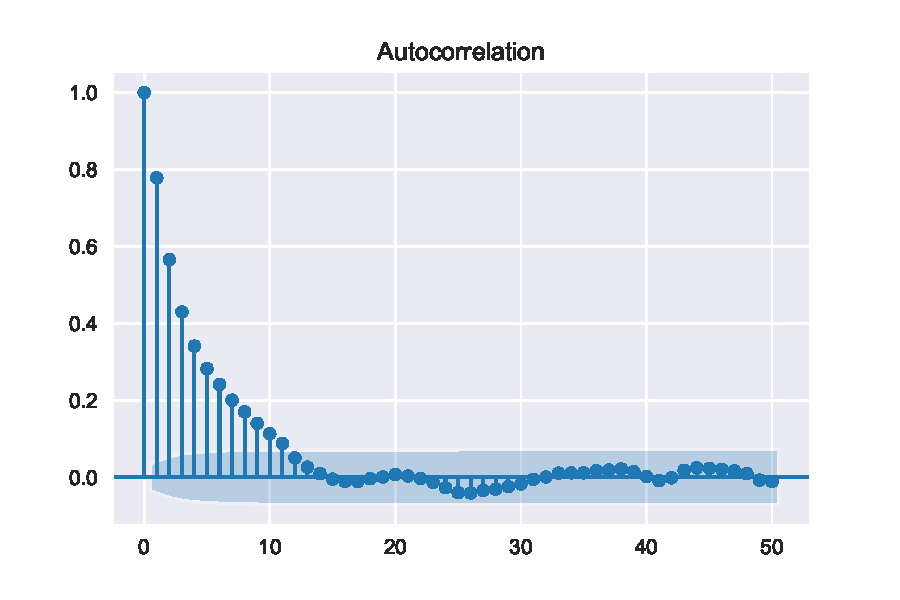
\includegraphics[scale=0.49]{acf2.pdf}
			\caption{Autokorelacja}
			\label{fig:acf2}
		\end{minipage}
		\begin{minipage}{0.49\linewidth}
			\centering
			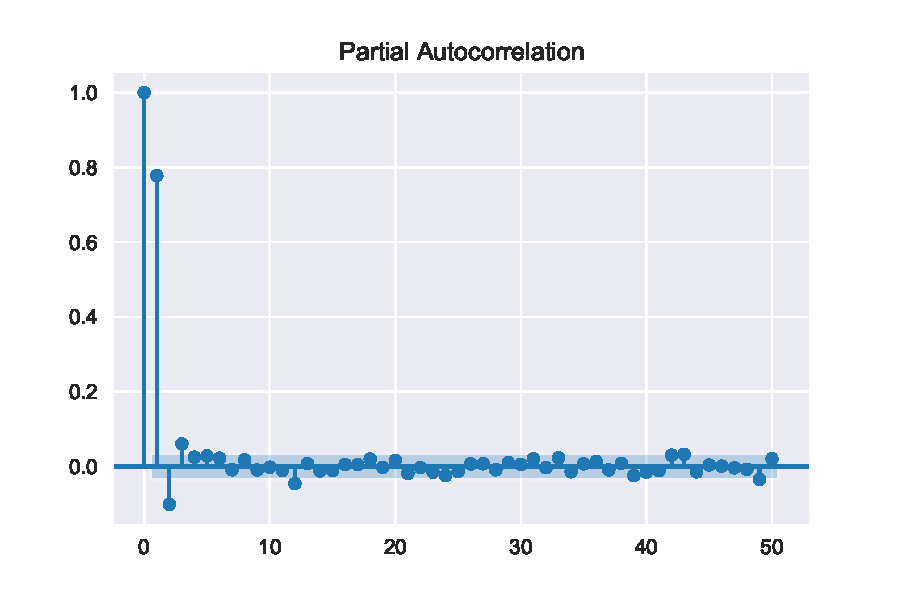
\includegraphics[scale=0.49]{pacf2.pdf}
			\caption{Częściowa autokorelacja}
			\label{fig:pacf2}
		\end{minipage}
	\end{center}
\end{figure}

\section{Ocena dopasowania modelu}

Musimy teraz dobrać rząd modelu ARMA(p,q). Do wykonania tego posłużą nam kryteria informacyjne.


\section{Weryfikacja założeń dotyczących szumu}




	\section{Podsumowanie}
	
	Na podstawie przeprowadzonej analizy możemy stwierdzić, że między poziomem szczęścia a PKB per capita dla danego kraju występuje dosyć silna zależność liniowa. Niestety badanie residuów wykazało, że nie mają one rozkładu normalnego. Oznacza to, że co prawda punktowe estymacje zostały przez nas wykonane poprawnie, jednak wszystkie estymacje przedziałowe oparte były o założenie o normalności rozkładu residuów, zatem nie mają zastosowania w tym modelu. Niestety nie znając rozkładu $\epsilon$, nie możemy wyznaczyć faktycznych przedziałów ufności.
	
	\section{Źródła}
	\begin{itemize}
		\item Wykłady
		\item \url{https://www.kaggle.com/datasets/eliasturk/world-happiness-based-on-cpi-20152020}
		\item \url{https://www.itl.nist.gov/div898/handbook/eda/section3/eda35a.html}
		\item \url{http://tofesi.mimuw.edu.pl/~cogito/smarterpoland/samouczki/testyNormalnosci/testyNormalnosci.pdf} str.11
		
	\end{itemize}
	
	
\end{document}